\documentclass{fefu_thesis/cls/fefu}

\usepackage{float}
\usepackage{caption}
\usepackage{subcaption}
\usepackage{hyperref}
\usepackage{algorithm}
\usepackage{algpseudocode}
\usepackage{amsmath}

\newenvironment{algo}[1][]
  {\begin{algorithm}[#1]
     \selectlanguage{english}
     \floatname{algorithm}{Алгоритм}
  }
  {\end{algorithm}}

\algdef{SE}[DOWHILE]{Do}{DoWhile}{\algorithmicdo}[1]{\algorithmicwhile\ #1}%

\newcommand*\gsegment[1]{\overline{#1}}
\newcommand*\gline[1]{\overleftrightarrow{#1}}
\newcommand*\gray[1]{\overrightarrow{#1}}
\newcommand*\talgref[1]{Алгоритм \ref{#1}}

\author{Терехов Дмитрий Евгеньевич}
\title{Полигонизация текстур и упаковка полигональных текстур в атлас}
\setfaculty{09.04.01 Информатика и вычислительная техника}
\setprogram{Искусственный интеллект и большие данные}
\setgroup{М9119-09.04.01иибд}
\setsupervisor{Сапрыкина Елена Валерьевна}{}
\setdirector{Мирин Илья Геннадьевич}{}
\setsecretary{Сапрыкина Елена Валерьевна}{}
\setpracticetitle{Преддипломная практика}
\addbibresource{references.bib}

\begin{document}
    \maketitle{practice}
    \begin{abstract}
        В данной работе представлены два эффективных алгоритма: генерация текстурного меша с последующим упрощением и упаковка полигональных текстур в атлас. Оба алгоритма работают с полигонами следующих типов: невыпуклые, полигоны с дырами, полигоны, состоящие из нескольких контуров.

        \textit{Ключевые слова: генерация меша, упрощение полигонов, упаковка в контейнеры.}
    \end{abstract}
    \pagebreak
    \tableofcontents
    \pagebreak
    {\centering\section*{Введение}}
    Целью работы является решение задач упрощения полигонов и упаковки, которые играют важную роль в таких прикладных областях, как компьютерная графика, GIS системы, промышленность и т.д. Решение этой задачи также опирается на прикладную область: компьютерную графику, а именно автоматическую генерацию текстурного меша с последующей упаковкой полигональных текстур в текстурные атласы.

    Упаковка в текстурные атласы это один из этапов подготовки ассетов-текстур для оптимального использования: маленькие текстуры становятся частью большого изображения -- текстурного атласа. Это позволяет минимизировать затраты по памяти, а также уменьшить количество вызовов на отрисовку. Текстурный меш позволяет уменьшить количество вызовов фрагментного шейдера (по сравнению с отрисовкой прямоугольника), путем минимизации площади пустых пикселей, входящих в меш. Представление текстур в виде полигонов позволяет упаковать больше текстур в атлас, так как в полигональном виде они занимают меньшую площадь.

    Не существует открытых программных пакетов или алгоритмов, которые решают поставленные задачи. Все программные пакеты являются проприетарными, а известные статьи решают данные задачи в очень упрощенном виде. Это и послужило мотивацией для проведения исследований и создания новых алгоритмов.

    В разделе <<Задачи упрощения полигонов и упаковки в контейнеры>> описывается важность поставленных задач для компьютерной графики и разработки игр, дается обзор теоретических положений и практических подходов к их решению.

    В разделе <<Алгоритмы, структуры данных и математические методы>> предлагается решение поставленных задач, приводится описание использованных и разработанных алгоритмов.

    В разделе <<Применение алгоритмов>> описывается применение результатов исследования в реальном игровом проекте компании <<Game Forest>>, разработанном на игровом движке с открытым исходным кодом <<Citrus>>.

    \section*{Глоссарий}
    \pagebreak
    \section{Задачи упрощения полигонов и упаковки в контейнеры}

    Целью работы является решение задач упрощения полигонов и упаковки, которые играют важную роль в таких прикладных областях, как компьютерная графика, GIS системы, промышленность и т.д. Решение этой задачи также опирается на прикладную область: компьютерную графику, а именно автоматическую генерацию текстурного меша с последующей упаковкой полигональных текстур в текстурные атласы.

    \subsection{Генерация текстурного меша}
    \label{TextureMeshGeneration}
    Полигональный меш (полигональная сетка) -- это совокупность вершин, рёбер и граней, которые определяют форму многогранного объекта в трёхмерной компьютерной графике и объёмном моделировании. В двумерной компьютерной графике меши используются для вершинной и скелетной анимации.

    \begin{figure}[H]
        \centering
        \includegraphics[scale=0.5]{images/spine_mesh.png}
        \caption{2D меш}
    \end{figure}

    Прежде чем объект попадет на экран, его текстуру и меш необходимо отправить на видеокарту, которые должны пройти этапы графического конвейера Рис. \ref{GraphicsPipeline}.

    \begin{figure}[H]
        \centering
        \includegraphics[scale=0.8]{images/graphicspipeline.png}
        \caption{Основные этапы графического конвейера}
        \label{GraphicsPipeline}
    \end{figure}

    Сначала для каждой вершины меша запускается вершинный шейдер, в котором вершины подвергаются различным преобразованиям (например, масштабирование или преобразование камеры). Далее необходимо растеризовать треугольник, то есть определить, какие пиксели на экране соответствуют данному треугольнику. Затем для каждого пикселя запускается пиксельный (или фрагментный) шейдер, который должен присвоить пикселю цвет (например, взятый из текстуры). Цвет полученного пикселя смешивается с цветом пикселя на экране. Стандартное уравнение смешивание цвета выглядит следующим образом:

    \[
        color = alpha \cdot pixelColor + (1 - alpha) \cdot color
    \]

    Из чего следует, что полностью прозрачные пиксели ($alpha = 0$) никак не влияют на цвет на экране.

    То, как объект попадает на экран, задает параметры качества для 2D меша: он должен состоять из как можно меньшего количества вершин и задевать минимальное количество прозрачных пикселей. Но алгоритма генерации качественного 2D меша или упрощения 2D меша нет.

    \begin{figure}[H]
        \centering
        \begin{subfigure}[c]{.49\linewidth}
            \centering
            \includegraphics{images/katana_rect.png}
            \caption{Прямоугольный меш с 4 вершинами}
        \end{subfigure}
        \begin{subfigure}[c]{.49\linewidth}
            \centering
            \includegraphics{images/katana_15v.png}
            \caption{Полигональный меш с 15 вершинами}
        \end{subfigure}
    \end{figure}

    В GIS системах возникает схожая задача: необходимо уменьшить количество вершин у кривой, задающей очертание береговой линии. Для этого разработали множество алгоритмов упрощения кривой: алгоритм Ramer–Douglas–Peucker \cite{Ramer}\cite{DouglasPeucker}, алгоритм радиального расстояния \cite{PolylineSimplification}, алгоритм Visvalingam–Whyatt \cite{VisvalingamWhyatt}, упрощение Opheim \cite{Opheim} и Lang \cite{Lang}, алгоритм Zhao–Saalfeld \cite{ZhaoSaalfeld}, алгоритм Reumann-Witkam \cite{ReumannWitkam}.

    Задачу упрощения 2D меша можно свести к задаче упрощения замкнутой кривой или же просто полигона, так как объединение треугольников меша является множеством простых полигонов с дырами. То есть можно без потери общности считать, что меш это -- триангуляция соответствующего ему множеству полигонов. Поэтому здесь и далее под задачей упрощения текстурного 2D меша будет подразумеваться задача упрощения полигонов.

    \begin{figure}[H]
        \centering
        \begin{subfigure}[c]{.49\linewidth}
            \centering
            \includegraphics{images/katana_15v.png}
            \caption{Меш}
        \end{subfigure}
        \begin{subfigure}[c]{.49\linewidth}
            \centering
            \includegraphics{images/katana_15v_polygon.png}
            \caption{Полигон}
        \end{subfigure}
    \end{figure}

    2D текстурный меш должен быть надмножеством контура изображения. Контур растрового изображения -- это множество последовательностей граничных пикселей. Меш, полученный из контура изображения, содержит в себе наибольшее количество вершин, но при этом не содержит в себе пустых пикселей.

    \begin{figure}[H]
        \centering
        \includegraphics[scale=1.2]{images/donutpixel_contour_none.png}
        \caption{Контур изображения}
    \end{figure}

    Полигоны, упрощенные алгоритмом упрощения кривых, могут нарушать свойство, изложенное выше. Также алгоритмы упрощения кривых не рассматривают задачу минимизации добавочной площади (или площади пустых пикселей). Их главным критерием качества является некая похожесть исходной кривой и упрощенной.

    Данная работа предлагает оригинальный алгоритм для упрощения контура изображения, который стремится минимизировать количество вершин и площадь пустых пикселей.

    \subsection{Упаковка текстур в атласы}

    Как было сказано в \ref{TextureMeshGeneration}, прежде чем отрисовать объект на экране, его текстуру и меш необходимо отправить на видеокарту. В компьютерной графике применяют различные подходы, которые позволяют уменьшить количество отправлений данных на GPU. Одним из таких подходов является использование текстурных атласов. Текстурный атлас -- это большое изображение, содержащее набор под-изображений. Под-текстуры отображаются на объект, используя UV-преобразование, при этом координаты в атласе задают, какую часть изображения нужно использовать. Если текстуры подряд идущих игровых объектов находятся в одном атласе, то при равенстве прочих параметров отрисовки (например, шейдеры или режим смешивания) эти объекты можно отрисовать разом за один Draw Call.

    \begin{figure}[H]
        \centering
        \includegraphics[scale=0.25]{images/texture_atlas_example.png}
        \caption{Текстурный атлас}
    \end{figure}

    Для того чтобы уменьшить размер текстур и ,соответственно, ускорить их загрузку на GPU, в компьютерной графике применяют компрессию. Алгоритмы сжатия часто ставят ограничение на размеры текстур. Например, размеры должны быть степенью двойки или даже длина должна совпадать с шириной. В этом случае текстуры, не подходящие под ограничения, необходимо изменить, что плохо сказывается на качестве текстуры или на её размере, поэтому при использовании компрессии целесообразно паковать текстуры в атлас.

    Упаковка текстур в атласы это частный случай задачи упаковки в контейнеры -- NP-трудной \cite{BinPackingIsNPHard} комбинаторной задачи. Задача заключается в упаковке объектов предопределённой формы в конечное число контейнеров предопределённой формы таким способом, чтобы число использованных контейнеров было наименьшим или количество или объём объектов (которые упаковывают) были наибольшими. В данной работе предлагается решение 2D irregular bin packing problem \cite{TypologyOfPackingProblems}, то есть упаковки полигональных объектов в прямоугольные контейнеры.

    Для упаковки прямоугольных объектов существует множество эвристических алгоритмов \cite{ThousandWayToPackBin}, которые хорошо показывают себя на практике.

    В области упаковки полигонов существуют различные подходы.

    No-fit polygon \cite{NofitPolygon}\cite{NofitPolygon2} -- это конструкция, которая определяет все положения, которые могут принимать два произвольных многоугольника относительно друг друга так, чтобы они соприкасались, но не перекрывались. Подсчет no-fit полигона необходимо производить для каждой вершины полигона и для каждой ориентации полигона, поэтому методы на основе no-fit polygon используют для решения задачи раскроя на производстве, где форма вырезаемых объектов несложная и заранее известна.

    Swarm intelligence (роевой интеллект) -- метод оптимизации, который описывает коллективное поведение децентрализованной самоорганизующейся системы: колонии светлячков \cite{FireFly}, муравьев \cite{AntColony}, пчел \cite{PlayrixArticle}, particle swarm optimization \cite{PSO}.

    Генетический алгоритм \cite{JAKOBS1996165} -- это эвристический алгоритм поиска, используемый для решения задач оптимизации и моделирования путём случайного подбора, комбинирования и вариации искомых параметров с использованием механизмов, аналогичных естественному отбору в природе.

    Существующие алгоритмы не удовлетворяют нужды упаковки текстур в атласы, поэтому данная работа предлагает оригинальную реализацию Memetic algorithm \cite{WhatIsMemetic} -- расширение генетического алгоритма, которое использует локальный поиск для уменьшения вероятности преждевременной сходимости. Разработанный алгоритм способен упаковывать изображения со свободным поворотом, на которых находятся множество разрозненных объектов с дырами.
    \pagebreak
    \section{Алгоритмы, структуры данных и математические методы}

    \subsection{Трассировка контура}
    Алгоритмы выделения контура можно разделить на 3 типа: обход попиксельно, обход повершинно, run-data.

    \begin{figure}[H]
        \centering
        \begin{subfigure}[t]{0.32\linewidth}
            \centering
            \includegraphics[scale=0.36]{images/pixel_following_algorithm.png}
            \caption{Обход попиксельно}
        \end{subfigure}
        \begin{subfigure}[t]{0.32\linewidth}
            \centering
            \includegraphics[scale=0.36]{images/vertex_following-algorithm.png}
            \caption{Обход повершинно}
        \end{subfigure}
        \begin{subfigure}[t]{0.32\linewidth}
            \centering
            \includegraphics[scale=0.36]{images/run_data_algorithm.png}
            \caption{Run data}
        \end{subfigure}
    \end{figure}

    \subsubsection{Обход попиксельно}

    Методы выделения контура начинаются с пикселя и обходят контуры изображения образом, специфичным для метода, а затем сохраняет их координаты в памяти в соответствии с порядком обхода. Наиболее известные алгоритмы обхода контура попиксельно: Moore-neighbor tracing \cite{MoorNeighbor}, radial sweep \cite{RadialSweep} и алгоритм Theo Pavlidis \cite{TheoPavlidis}.

    \subsubsection{Обход повершинно}

    Метод выделения контура обходом повершинно отличается от обхода попиксельно лишь тем, что обход осуществляется по границам пикселей.

    \subsubsection{Run-data}

    Run-data методы выделения контура проходят по изображению сканирующей линией, оставляя зависящие от конкретного алгоритма метки на встреченном граничном пикселе. Далее, по расставленным меткам восстанавливается контур изображения. Примеры методов этой группы: run-type direction code \cite{Miyatake1997}, методы, основанные на PXY таблице \cite{Shoji}. Отличительной особенностью run-data методов является возможность выделения внешних и внутренних контуров, сохраняя иерархию. Так же способ обхода изображения в некоторых алгоритмах позволяет не держать в памяти изображение целиком.

    Было решено выбрать алгоритм именно из этой группы методов, так как необходимо выделять дырки на объектах. За основу был взят алгоритм Suzuki Satoshi \cite{SuzukiAlgorithm}, использующийся в библиотеке OpenCV. Алгоритм способен построить иерархию контуров и типизировать их на границы и дыры.

    \begin{figure}[H]
        \centering
        \begin{subfigure}[t]{.49\linewidth}
            \includegraphics[scale=0.4]{images/SuzukiExample_upscaled.png}
            \caption{Изображение}
        \end{subfigure}
        \begin{subfigure}[t]{.49\linewidth}
            \includegraphics[scale=0.4]{images/SuzukiExample_contours_upscaled.png}
            \caption{Контуры изображения}
        \end{subfigure}
        \begin{subfigure}[t]{.99\linewidth}
            \centering
            \includegraphics[scale=0.7]{images/SuzukiExample_hierarchy.png}
            \caption{Иерархия контуров}
        \end{subfigure}
        \caption{Пример работы алгоритма Suzuki Satoshi}
    \end{figure}

    Алгоритм оперирует с дискретными координатами пикселей, а в компьютерной графике UV координаты это непрерывные вещественные числа. Такое представление контура создает некоторые проблемы.

    Во-первых, может получится контур с самопересечениями, которые нетривиально разрешить. На Рис. \ref{SelfIntersectingContours} изображены примеры контуров с самопересечением. Красным обозначены вершины, которые алгоритм посещает дважды.
    \begin{figure}[H]
        \centering
        \begin{subfigure}[t]{.49\linewidth}
            \centering
            \includegraphics[scale=0.2]{images/SelfIntersectingContour1.png}
            \caption{Изображение}
        \end{subfigure}
        \begin{subfigure}[t]{.49\linewidth}
            \centering
            \includegraphics[scale=0.4]{images/SelfIntersectingContour2.png}
            \caption{Контуры изображения}
        \end{subfigure}
        \caption{Примеры контуров с самопересечением}
        \label{SelfIntersectingContours}
    \end{figure}

    Во-вторых, некоторые пиксели при отрисовке будут обрезаны, так как дискретные координаты пикселя в прямой интерпретации в качестве UV координат будут являются координатами левого верхнего угла пикселя. В таком случае, нижние и правые пиксели просто не будут учтены при отрисовке.

    \begin{figure}[H]
        \centering
        \begin{subfigure}[t]{.33\linewidth}
            \centering
            \includegraphics[scale=0.2]{images/SuzukiExample2.png}
            \caption{Изображение}
        \end{subfigure}
        \begin{subfigure}[t]{.33\linewidth}
            \centering
            \includegraphics[scale=0.2]{images/SuzukiExample2_uvs.png}
            \caption{Контуры изображения + UV координаты}
        \end{subfigure}
        \begin{subfigure}[t]{.32\linewidth}
            \centering
            \includegraphics[scale=0.2]{images/SuzukiExample2_wanted_uvs.png}
            \caption{Контур изображения и желаемые UV координаты}
        \end{subfigure}
        \caption{Проблема неправильных UV координат}
    \end{figure}

    Для решения данных проблем был разработан алгоритм, который превращает попиксельный контур в повершинный.
    \begin{algo}[H]
        \setstretch{1}
        \caption{Pixel contour to vertex contour}
        \begin{algorithmic}[1]
            \State $C$ is an ordered contour
            \State $p \gets$  top left vertex of $C_0$
            \State $texel \gets C_0$ is a current texel coordinates (correspond to texel center)
            \State $TraceTexel$ traces all vertices of $texel$ in a CCW order until the vertex of $nextTexel$ is met
            \For{$i$ \textbf{from} 1 \textbf{to} $\left|C\right| - 1$}
                \State $nextTexel \gets C_i$
                \State $p \gets TraceTexel\left(p, texel, nextTexel\right)$
                \State $texel \gets nextTexel$
            \EndFor
            \State $TraceTexel\left(p, texel, C_0\right)$
            \State Resulting vertex contour consists of all traced vertices
        \end{algorithmic}
    \end{algo}

    Зная локальные координаты вершины относительно текселя, можно легко определить как принадлежность вершины к текселю, так и следующую вершину против часовой стрелки. Для перехода к локальным координатам нужно отнять координаты текселя. Вершина принадлежит текселю, если локальные координаты относительно текселя удовлетворяют неравенству $ 0 \leq x, y \leq 1$.

    \begin{figure}[H]
        \centering
        \begin{subfigure}[t]{.49\linewidth}
            \centering
            \includegraphics[scale=0.8]{images/texel_vertex_absolute.png}
            \caption{Абсолютные координаты}
        \end{subfigure}
        \begin{subfigure}[t]{.49\linewidth}
            \centering
            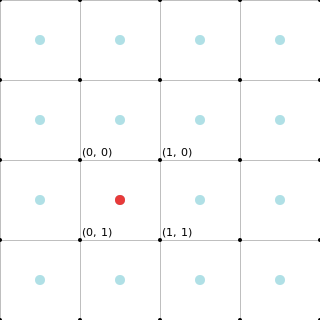
\includegraphics[scale=0.8]{images/texel_vertex_local.png}
            \caption{Локальные координаты относительно текселя $\left(1, 2\right)$}
        \end{subfigure}
        \caption{Переход к локальным координатам}
    \end{figure}

    Переход к следующей вершине против часовой стрелки может осуществляться с помощью простой табличной функции:

    \begin{fefutable}[H]{|c|c|c|}{Функция следющей вершины против часовой стрелки}
        \hline
        $x\textbackslash y$& $0$ & $1$\\
        \hline
        $0$ & $\left(0, 1\right)$ & $\left(1, 1\right)$\\
        \hline
        $1$ & $\left(0, 0\right)$ & $\left(1, 0\right)$\\
        \hline
    \end{fefutable}

    Для того, чтобы снизить количество вершин перед следующим этапом обработки изображения, контуры подвергаются первичной аппроксимации. Самым очевидным способом аппроксимации контура является удаление вершин лежащих на одной прямой. Также существуют алгоритмы упрощения цифровых кривых. В данной работе был реализован алгоритм Teh-Chin\cite{TehChin} c $L1$ и $k\cos$ метриками.

    \subsection{Аппроксимация полигонов}
    \label{PolygonApproximation}

    Аппроксимация полигонов для текстурных мешей отличается от аппроксимации кривых, например, в GIS системах: аппроксимированный полигон должен быть надмножеством исходного, а так же необходимо минимизировать не только количество вершин, но и добавочную площадь.

    Разработанный алгоритм действует следующим образом. Для каждой вершины рассчитываются возможные трансформации. Каждая трансформация удаляет одну вершину, но добавляет некоторую площадь, занимаемую прозрачными пикселями. Эта добавочная площадь является стоимостью преобразования. На каждом шаге алгоритм либо выполняется минимальное преобразование среди всех вершин, либо сливает два полигона в один. Так происходит до тех пор, пока не будет достигнуто условие выхода либо невозможно будет выполнить шаг алгоритма.

    Полигон $P_i$ представляется двусвязным зацикленным списком вершин $P_i = \left(v_j\right)_{j=0}^{n - 1}$. Здесь и далее обозначение $v_{j \pm m}$ обозначает взятие по модулю $v_{j \pm m \pmod n}$.

    \subsubsection{Преобразования над вершинами}
    Рассмотрим возможные преобразования над вершинами.

    \paragraph{Удаление вершин, лежащий на одной прямой}

    Данная трансформация имеет нулевую стоимость и проста в реализации.

    \paragraph{Удаление вогнутого/выпуклого угла}

    Если вершина $v_i$ принадлежит границе или дыре и образует вогнутый или выпуклый угол соответственно, то возможно провести отрезок $\gsegment{v_{i - 1}v_{i + 1}}$ и удалить вершину $v_i$. Также из теоремы о двух ушах \cite{TwoEars} следует, что любой последовательностью  таких преобразований можно сократить дыру до треугольника. Теорема о двух ушах гласит, что в каждом простом полигоне с более чем 3 вершинами есть хотя бы 2 уха. Ухом называется вершина, соседние вершины которой можно соединить отрезком, который будет полностью лежать внутри полигона.

    \begin{figure}[H]
        \centering
        \includegraphics[scale=1]{images/earcut.png}
        \caption{Удаление вогнутого угла}
    \end{figure}

    \paragraph{Частичное удаление вогнутого угла}

    Данное преобразование является качественной версией удаления вогнутого угла (имеет меньшую стоимость). Если $\gray{v_{i - 2}v_{i - 1}}$ пересекает $\gsegment{v_iv_{i + 1}}$, то можно не отрезать весь угол, а заменить $v_{i - 1}$ и $v_{i}$ пересечением. Аналогично работает для $\gray{v_{i + 2}v_{i + 1}}$ и $\gsegment{v_iv_{i - 1}}$.

    \begin{figure}[H]
        \centering
        \includegraphics[scale=1]{images/bendneighbor.png}
        \caption{Выгибание соседней вершины}
    \end{figure}

    \paragraph{Пересечение сторон}

    Если $v_i$ образует выпуклый угол, то может существовать возможность заменить вершину $v_i$ и $v_{i + 1}$ пересечением $\gray{v_{i - 1}v_i}$ и $\gray{v_{i + 2}v_{i + 1}}$.

    \begin{figure}[H]
        \centering
        \includegraphics[scale=1]{images/bendneighbor2.png}
        \caption{Пересечение сторон}
    \end{figure}

    \paragraph{Выгибание двух соседних вершин}

    Пусть $v_{i - 1}$, $v_{i}$ и $v_{i + 1}$ являются вершинами выпуклых углов, тогда можно попробовать заменить все 3 вершины пересечением $\gray{v_{i - 2}v_{i - 1}}$ и $\gray{v_{i + 2}v_{i + 1}}$ с вертикальной или горизонтальной прямой, проходящей через $v_i$.

    \begin{figure}[H]
        \centering
        \includegraphics[scale=1]{images/bendoutboth.png}
        \caption{Выгибание двух соседних вершин к вертикальной прямой}
    \end{figure}

    \paragraph{Удаление треугольной дыры}

    Если дыра упростилась до треугольника и внутри нет граничных полигонов, то единственная возможная трансформация для этих вершин -- удаление всей треугольной дыры.

    \begin{figure}[H]
        \centering
        \includegraphics[scale=1]{images/remove_triangular_hole.png}
        \caption{Удаление треугольной дыры}
    \end{figure}

    \subsubsection{Слияние полигонов}

    В каждой полигональной дыре выбирается 2 пары последовательных вершин из разных полигонов, которые образуют минимальный четырехугольник, который не пересекает другие стороны. Данные 4 вершины являются точками слияния.

    \begin{figure}[H]
        \centering
        \begin{subfigure}[t]{\linewidth}
            \centering
            \includegraphics[scale=1]{images/polygonmerge.png}
            \caption{Слияние границы с дырой}
        \end{subfigure}
        \begin{subfigure}[t]{\linewidth}
            \centering
            \includegraphics[scale=1]{images/polygonmerge2.png}
            \caption{Слияние границы с границей}
        \end{subfigure}
    \end{figure}

    Нахождение пар точек для потенциального слияния осуществляется с помощью сопоставления полигонов видимости. Полигон видимости для точки $p$ это полигональная область точек плоскости, видимых из точки $p$.

    \begin{figure}[H]
        \centering
        \includegraphics[scale=0.35]{images/visibility_polygon.png}
        \caption{Полигон видимости}
    \end{figure}

    На Рис. \ref{VP} показаны полигоны видимости двух соседних вершин. Красным отмечена вершина запроса. Фиолетовым отмечены интересующие нас вершины, через которые можно потенциально слить полигоны. Серым отмечены либо вершины, принадлежащие тому же полигону, что и вершина запроса, либо точки, не являющиеся вершинами полигона.

    \begin{figure}[H]
        \centering
        \begin{subfigure}[t]{0.49\linewidth}
            \centering
            \includegraphics[scale=0.5]{images/visibility_polygon_current_vertex.png}
            \caption{Полигон видимости текущей вершины}
        \end{subfigure}
        \begin{subfigure}[t]{0.49\linewidth}
            \centering
            \includegraphics[scale=0.5]{images/visibility_polygon_prev_vertex.png}
            \caption{Полигон видимости предыдущей вершины}
        \end{subfigure}
        \caption{Полигоны видимости соседних вершин}
        \label{VP}
    \end{figure}

    Пусть у нас есть вершины 2 последовательные вершины $prev$ и $current$ некоторого полигона $P$. Также для них известны полигоны видимости $V_{prev}$ и $V_{current}$. Тогда для каждой точки $q \in V_{current}$, являющийся вершиной полигона, но $q \notin P$, необходимо проверить, $next\left(q\right) \in V_{prev}$. Если $next\left(q\right) \in V_{prev}$, значит 2 полигона можно слить через вершины $prev, next\left(q\right), q, current$, проверив при этом отсутствие самопересечения. Запрос о нахождении точки в полигоне видимости можно выполнить за $O\left(\log \left|V\right|\right)$ при помощи бинарного поиска, так как вершины полигона видимости отсортированы по полярному углу относительно точки запроса.

    \begin{algo}[H]
        \setstretch{1}
        \caption{Can merge polygon with other through given two consecutive vertices}
        \begin{algorithmic}[1]
            \State $current,\;prev$ are two consecutive vertices of $P$
            \State $vp \gets FindVisibilityPolygon\left(current\right)$
            \State $pvp \gets FindVisibilityPolygon\left(prev\right)$
            \State $minArea \gets \infty$
            \State $minPair \gets None$
            \For{$v \in vp$}
                \If{$v \in P$ \textbf{or} $v$ \textbf{is not} vertex of any other polygon}
                    \State \textbf{continue}
                \EndIf
                \State $Q \gets PolygonOf\left(v\right)$
                \State $vNext \gets NextVertex(Q,\;v)$
                \If{$vNext \in pvp$ \textbf{and} $\gsegment{prev, current} \cap \gsegment{v, vNext} =\emptyset$}
                    \State $area \gets AreaOfQuadrilateral\left(prev,\;current,\;v,\;vNext\right)$
                    \If{$area < minArea$}
                        \State $minArea \gets area$
                        \State $minPair \gets \left(v,\;vNext\right)$
                    \EndIf
                \EndIf
            \EndFor
            \State \textbf{return} $minPair$
        \end{algorithmic}
    \end{algo}

    В данной работе был реализован алгоритм Triangular Expansion \cite{TriangularExpansion} для нахождения полигона видимости в триангуляции. Данный алгоритм для точки запроса $q$ в полигоне $P$ сначала находит треугольник, содержащий точку. Очевидно, что $q$ видит весь треугольник и к полигону видимости можно добавить все ребра, которые принадлежат $\partial P$. Для всех других ребер вызывается рекурсивная процедура, которая расширяет поле зрения $q$ через ребро. Изначально поле зрения $q$ ограничивается концами ребра, однако по мере углубления в рекурсию, поле зрения может быть дополнительно ограничено. Алгоритм затрачивает $O\left(nh\right)$ времени и $O\left(n\right)$ памяти, где $h$ это количество дыр. Но на практике алгоритм часто затрачивает сублинейное время, так как затрагивает только треугольники, которые на самом деле видны.

    \subsubsection{Применение преобразований}

    В данном алгоритме используется триангуляция Делоне с ограничениями в качестве одного из представлений множества полигонов. Ограниченные ребра задают границы полигонов. Операции над триангуляцией Делоне позволяют эффективно проверять возможность трансформации. Вставка вершин и структурных ребер позволяет проверить возможность совершения геометрического преобразования, а проверка на наличие треугольника  позволяет проверить случаи, когда преобразование полностью включает в себя сторонний полигон (Рис. \ref{TriangleExistenceCheck}). Для построения триангуляции используется программный пакет \cite{Terekhov}, разработанный автором.

    \begin{figure}[H]
        \centering
        \includegraphics[scale=1]{images/triangle_existance_check.png}
        \caption{Проверка на наличие треугольника}
        \label{TriangleExistenceCheck}
    \end{figure}

    Вершины дополнительно хранятся в двоичном дереве поиска, отсортированной по стоимости их преобразования. На каждой итерации цикла применяется аппроксимирующее преобразование с минимальной стоимостью. После применения преобразования пересчитываются преобразования соседних вершин. Аппроксимация соседних контуров или объемлющей дыры могут повлиять на валидность посчитанного преобразования. При неудачной попытке произвести преобразование, преобразование для вершины пересчитывается, берется новая вершина из дерева и попытки повторяются. Такой ленивый пересчет позволяет избежать больших временных затрат, так как любая трансформация может в худшем случае повлиять на трансформацию $O\left(n\right)$ вершин. Однако на практике такое встречается редко.

    \subsubsection{Вычислительная устойчивость}

    Вычислительная устойчивость алгоритма достигается использованием вычислительно устойчивых геометрических предикатов, разработанных Jonathan\\Shewchuk \cite{shewchuk97a}. Данные предикаты также используются для построения Делоне с ограничениями.

    \subsubsection{Меш}

    Для отрисовки объектов в игре понадобится получить текстурный меш из аппроксимированного контура. Так как для аппроксимации создается триангуляция Делоне, то необходимо просто выбрать из неё нужные треугольники. Для этого достаточно запустить обход в глубину триангуляции. Основой триангуляции является структура данных Halfedge \cite{Halfedge}, представляющая собой ориентированное ребро с указателем на следующее и соседнее, ориентированное в обратном направлении, ребро. Каждое ограниченное ребро триангуляции является ребром одного из полигонов. Значит, при переходе через такое ребро мы входим или выходим в/из площади объекта на картинке.

    \begin{algo}[H]
        \setstretch{1}
        \caption{Retrieve image mesh}
        \begin{algorithmic}[1]
            \State $used \gets \emptyset$
            \State $faceList \gets []$ a list of indices triplets
            \Procedure{RetrieveMesh}{$edge, faceIndices, faceList$}
                \If{$faceIndices \neq null$} \Comment{Means inside a polygon}
                    \State $faceIndices \gets faceIndices \bigcup \left|faceList\right|$
                    \State $faceList \gets faceList \bigcup FaceFrom\left(edge\right)$
                \EndIf
                \State $current \gets edge.Next$
                \State $used \gets used \cup current$
                \State $used \gets used \cup current.Next$
                \State $used \gets used \cup current.Prev$
                \While{$current \neq edge$} \Comment{Recursively call to other sides}
                    \If{$current.Twin \neq null \; \textbf{and} \; used \cap current.Twin != \emptyset$ }
                        \State $twin \gets current.Twin$
                        \State $fis \gets faceIndices$
                        \If{$twin.IsConstrained$} \Comment{We enter or leave polygon}
                            \State $fis \gets $ face indices that correspond to entering polygon or null if leaving
                        \EndIf
                        \State $RetrieveMesh(twin, fis, faceList)$
                    \EndIf
                \EndWhile
                \State $current \gets current.Next$
            \EndProcedure
        \end{algorithmic}
    \end{algo}

    \subsection{Генетический алгоритм}

    Основная идея всех эволюционных алгоритмов одинакова: популяция особей в некоторой среде конкурирует за ограниченные ресурсы, конкуренция приводит к естественному отбору -- выживает наиболее приспособленный. Каждая особь представляет собой элемент в области определения функции приспособленности (fitness or evaluation function, функции оценки), которую необходимо минимизировать. Изначально создается популяции из случайных значений из области определения функции. Затем отбираются лучшие особи, которые подвергаются воздействию операторов вариации (рекомбинации и\textbackslash или мутации). Из полученной популяции только часть наиболее приспособленных особей доживает до нового поколения. И так повторяется до тех пор, пока не будет достигнуто желаемое решение. Генетический мета-алгоритм показан в \talgref{meta-genetics}.

    \begin{algo}[H]
        \setstretch{1}
        \caption{Генетический мета-алгоритм}
        \label{meta-genetics}
        \begin{algorithmic}[1]
            \State $INITIALIZE$ population with random candidate solution
            \State $EVALUATE$ each candidate
            \While{$TERMINATION\; CONDITION$ \textbf{is not} satisfied}
                \State $SELECT$ parents
                \State $RECOMBINE$ pairs of parents
                \State $MUTATE$ offspring
                \State $EVALUATE$ new candidates
                \State $SELECT$ individuals for the next generation
            \EndWhile
        \end{algorithmic}
    \end{algo}

    Стоит отметить, что все компоненты, кроме оценки особей, являются стохастическими. Например, мутация задевает случайную часть решения, а слабые особи имеют малый шанс выиграть в естественном отборе.

    \subsubsection{Составные части генетического алгоритма}

    \paragraph{Инициализация}

    Чаще всего изначальная популяция просто заполняется случайно сгенерированными особями. Однако, могут использоваться специфические для данной проблемы эвристики, которые позволяют создать более приспособленную изначальную популяцию.

    \paragraph{Функция оценки}

    Функция оценки задает требования, к которым популяция вынуждена адаптироваться. Технически, это функция, которая определяет меру качества особи. Смысл всего генетического алгоритма в минимизации функции оценки для популяции, чтобы достичь наиболее качественного решения.

    \paragraph{Популяция}

    Популяции -- это набор особей. Практически во всех вариантах эволюционных алгоритмов размер популяции постоянен. Отбор берет во внимание всю популяцию целиком, а не отдельно каждого индивида.

    \paragraph{Механизм отбора родителей}

    Механизм отбора родителей используется, чтобы выбрать наиболее хороших особей для того, чтобы они стали родителями для следующего поколения. Отбор родителей необходим, чтобы повысить качество будущего поколения. Для создания потомства к родителям применяют операторы вариации. Выбор родителей всегда вероятностный. Более приспособленные особи имеют высокий шанс стать родителями. Менее приспособленным особям тоже дается шанс, но малый, иначе поиск решения будет слишком жадным.

    \paragraph{Операторы вариации. Мутация и рекомбинация}

    Ролью операторов вариации является создание новых особей из старых. Операторы вариации разделяют на 2 группы по арности: унарная и n-арная версии. Все операторы вариации, обычно, стохастические. Исключением является применение операторов вариации, в которых заложено знание о проблеме. Таким образом, можно исключить образование заведомо неверных решений в популяции либо всегда создавать решения лучше их родительских.

    Унарный оператор вариации называют мутацией. Мутация применяется к одной особи, производя из неё новую слегка измененную особь. Роль мутации заключается в исследовании новых мест в области значений функции оценки. Мутация позволяет избежать преждевременной сходимости в локальном минимуме.

    Бинарный оператор вариации называют рекомбинацией или кроссовером. Как следует из названия, такой оператор совмещает информацию от двух родителей, сохраняя свойства от обоих. Роль кроссовера заключается в эксплуатации области значения функции оценки, занимаемой текущим поколением популяции.

    \paragraph{Механизм отбора выживших}

    После создания новых особей необходимо выбрать, какие особи составят следующее поколение популяции. Как и механизм отбора родителей, механизм отбора выживших является стохастическим и дает шанс менее приспособленным особям быть отобранными в новое поколение.

    \paragraph{Условие выхода}

    Условие выхода очень сильно зависит от задачи. Часто используют следующие варианты или их комбинации:

    \begin{itemize}
        \item Популяция сошлась к какому-то решение;
        \item Было достигнуто достаточно качественное решение;
        \item Был достигнут лимит времени на эволюцию;
        \item Прирост качества сильно замедлился;
        \item и т.д.
    \end{itemize}

    \subsection{Упаковка в атлас}

    Для упаковки в атлас мы используем классический генетический алгоритм из \talgref{meta-genetics}, но с некоторыми модификациями, о которых будет сказано позже. Для начала перечислим конкретные имплементации всех этапов генетического алгоритма для упаковки полигональных изображений в атлас.

    \subsubsection{Репрезентация особей}
    Особь представляет из себя решение задачи об упаковке для заданного размера атласа и набора изображений. Каждое изображение это набор объектов, которые из себя представляют под-меш изображения.

    \begin{figure}[H]
        \centering
        \includegraphics[scale=0.7]{images/Image.png}
        \caption{Структуры данных Image и ImageObject}
    \end{figure}

    Особь состоит из 2 массивов данных. В первом массиве хранятся тройки целых чисел, отвечающие за трансформацию каждого $ImageObject$ (перемещение по осям X и Y, а также поворот вокруг центроида). Во втором массиве хранятся флаги присутствия конкретного $Image$ в атласе ($true$ -- присутствует, $false$ -- отсутствует). Это обусловлено тем, что всё изображение целиком должно входить в атлас, при этом его части могут быть упакованы в разные места атласа.

    \subsubsection{Популяция}

    Размер популяции константный и задается в качестве параметра для генетического алгоритма.

    \subsubsection{Механизм отбора родителей}

    Как было сказано ранее, отбор родителей -- это стохастический процесс, в котором более приспособленные родители имеют более высокий шанс быть выбранными, поэтому первое, что приходит на ум, это присвоить шанс выбора пропорционально значению функции оценки, то есть $P\left(i\right) = \frac{f_i}{\sum_{j=0}^{n - 1} f_i}$. Однако такое наивное решение имеет ряд недостатков:

    \begin{itemize}
        \item Выдающиеся особи быстро захватывают популяцию, что вырождается в преждевременной сходимости, часто, не к лучшему результату;
        \item Когда значение оценочной функции особей близко друг к другу, то выбор становится равномерно случайным;
        \item При применении аффинных преобразований к функции оценки, данный способ отбора начинает вести себя совершенно по-другому.
    \end{itemize}

    Отбор по рангу\cite{RankingSelection} это другой метод, вдохновленный недостатками отбора по значению оценочной функции. Данный метод сортирует популяцию по значению оценочной функции и присваивает ранг каждой особи (лучшее решение имеет ранг $n - 1$, а худшее $0$). Вероятность отбора вычисляется на основе ранга, например, линейно или экспоненциально уменьшаясь от лучшего решения к худшему,

    \begin{align*}
        P_{linear}\left(i\right) &= \frac{2 - s}{n} + \frac{2i\left(s - 1\right)}{n\left(n - 1\right)},\\
        P_{exp}\left(i\right) &= \frac{1 - e^{-i}}{c},
    \end{align*}

    где $s$ это константа $1 < s\leq 2$, а $c$ выбирается так, чтобы сумма вероятностей равнялась $1$. В алгоритме упаковки применяется отбор по рангу с экспоненциальной формулой.

    После присвоения вероятностей выбора каждой особи необходимо составить множество родителей. Для этого существуют такие алгоритмы, как roulette wheel или tournament selection, но в алгоритме упаковки было решено использовать \textbf{stochastic universal sampling}\cite{RankingSelection}.

    \begin{algo}[H]
        \setstretch{1}
        \caption{Stochastic Universal Sampling}
        \begin{algorithmic}[1]
            \State $a$ is cumulative probability distribution
            \State $m$ is number of parents we want to selects
            \State $current \gets 1$
            \State $i \gets 1$
            \State $r \gets$ uniformly random from $\left[0, 1 / m\right]$
            \While{$current \leq m$}
                \While{$r \leq a_i$}
                    \State $parents_i \gets popoluation_i$
                    \State $r \gets r + 1 / m$
                    \State $current \gets current + 1$
                \EndWhile
                \State $i \gets i + 1$
            \EndWhile
        \end{algorithmic}
    \end{algo}

    \subsection{Мутация}
    В алгоритме упаковки равновероятностно выбирается одна из двух мутаций: \textbf{Reset} и \textbf{Creep}.

    \textbf{Random Resetting} мутация изменяет значение случайного гена на значение из заранее определенного диапазона. Например, ген вращения $ImageObject$ можно повторно установить в значение в диапазоне $\left[0, 359\right]$ градусов.

    \textbf{Creep} мутация добавляет какую-то малую случайную дельту к значению гена. Например, можно добавлять к гену поворота случайный поворот в диапазоне $\left[-10, 10\right]$ градусов.

    \subsection{Кроссовер}

    В алгоритме упаковки используется простейший одноточечный кроссовер, работу которого демонстрирует следующее изображение.

    \begin{figure}[H]
        \centering
        \includegraphics[scale=1]{images/OnePointCrossover.png}
        \caption{Одноточечный кроссовер}
    \end{figure}

    \subsection{Отбор выживших}
    В алгоритме используется композитная стратегия отбора выживших, состоящая из следующих стратегий отбора.

    \textbf{Age based}. Если особь прожила больше $a$ поколений, то эта особь не попадает в новое поколение.

    \textbf{Elitism}. $e$ наиболее приспособленных особей обязательно проходят в следующее поколение. Данная стратегия позволяет не потерять наиболее хорошее решение из найденных.

    \textbf{Replace worst (GENITOR)}. $m$ худших особей замещаются созданными потомками.

    \subsection{Функция оценки}

    Функция оценки включает в себя ограничения, накладываемые на решение, и задана таким образом, чтобы мотивировать популяцию эволюционировать в приемлемое решение как можно быстрее. Главными ограничениями является площадь пересечения полигонов и площадь выступов, образуемых минимальными и максимальными значениями координат $ImageObject$.

    \begin{figure}[H]
        \centering
        \includegraphics[scale=0.5]{images/ledges.png}
        \caption{Площадь выступов}
    \end{figure}

    Эти два ограничения мотивируют решение строиться таким образом, чтобы все фигуры попадали в атлас и не пересекались с остальными фигурами. Также в функции оценки учитывается площадь изображений, не попавших в атлас, что мотивируют решение вобрать себя как можно больше изображений. Функция оценки -- это сумма перечисленных выше слагаемых с коэффициентами:
    \[
        F\left(individual\right) = a \cdot S_{intersection} + b \cdot S_{outside\;ledges} + c \cdot S_{missing}
    \]
    где $c$ это коэффициент, контролируемый снаружи. С его помощью можно ослабить требование к решению, что позволит алгоритму сойтись.

    Если нахождение второго и третьего слагаемых тривиально, то нахождение площади пересечения всех полигонов довольно сложно. Существуют алгоритмы, способные производить булевые операции над полигонами с дырами и самопересечениями. Например, алгоритмы Vatti \cite{Vatti}, Greiner-Hormann \cite{GreinerHormann} или Martinez \cite{Martinez}. В данной работе был реализован модифицированный алгоритм Martinez \cite{Martinez}, способный подсчитать за один проход объединение всех полигонов, однако в скорости он всё равно уступает библиотеке Clipper за авторством Angus Johnson \cite{Clipper}, которая представляет собой расширение алгоритма Vatti \cite{Vatti}. Площадь пересечения между фигурами считается, как разница площади объединения и суммы площади полигонов $S_{intersection} = S\left(\bigcup\limits_{i = 0}^{m - 1} P_i\right) - \sum\limits_{i = 0}^{m - 1}S\left(P_i\right)$.

    \subsection{Memetic algorithm}

    Данный алгоритм упаковки является расширением классического генетического алгоритма, представленного в \talgref{meta-genetics}, и является реализацией memetic algorithm, который использует процедуру локального поиска, именуемой в литературе фазой обучения (learning phase). Некоторые выбранные особи перед отбором родителей проходят процедуру локального поиска, которой известна специфика решаемой проблемы и которая пытается улучшить существующее решение. В данной работе используются 2 процедуры локального поиска: \textbf{hole filling} и \textbf{physics}.

    \textbf{Hole filling}. Процедура пытается заполнить полигональные дыры объектами, которые потенциально могут поместиться в данную дыру.

    \textbf{Physics}. Используется симуляция физики при помощи известного физического движка Box2D \cite{Box2D}. Симуляция физики позволяет быстро преодолеть момент, когда между объектами остаются маленькие пересечения, от которых долго избавляется эволюция.

    \subsection{Условие выхода}
    Условие выхода имеет 2 этапа. Первый этап -- это достижение приемлемого решения. Решение считается приемлемым, если $S_{outside_ledges} = S_{intersection} = 0$. Далее дается константное количество поколений для улучшения решения.

    Условие выхода может сработать, когда ещё не все изображения упаковались (возможно, их и нельзя упаковать в тот же атлас). Для неупакованных изображений алгоритм запускается заново.

    \subsection{Выбор размера атласа}

    Размер атласа выбирается путем упаковки изображений быстрым жадным алгоритмом. Например, алгоритмом гильотины \cite{ThousandWayToPackBin}.
    \pagebreak
    \section{Применение алгоритмов}


    Алгоритмы нашли применение в продуктах компании <<Game Forest>>.

    \subsection{Game Forest}

    \begin{figure}[H]
        \centering
        \includegraphics[scale=0.25]{images/GF.png}
    \end{figure}

    <<Game Forest>> -- студия разработки мобильных free to play игр. За 15 лет студия создала свыше 40 игр, общая аудитория которых —  около 100 миллионов человек по всему миру. В числе проектов, над которыми работала компания, есть такие хиты, заслужившие всеобщее признание и высокие оценки пользователей, как:

    \begin{itemize}
      \item Midnight Mysteries --- лучшая инновационная игра 2010 года по версии Big Fish Games;
      \item 7 Wonders: Magical Mystery Tour — в ТОП 10 игр 2011 года по версии Microsoft;
      \item Midnight Mysteries: Ghostwriting --- номинации Best Story и Best Concept 2015 года от сайта All About Casual Game;
      \item Gummy Drop --- один из мировых лидеров в жанре Match-3 в настоящее время.
    \end{itemize}

    \subsection{Citrus}

    \begin{figure}[H]
        \centering
        \includegraphics[scale=0.4]{images/Citrus.png}
    \end{figure}

    Свои игры компания разрабатывает на игровом движке с открытым исходным кодом Citrus.  Citrus состоит из следующих компонент:

    \begin{itemize}
      \item Yuzu --- библиотека, предоставляющая средства сериализации;
      \item Kumquat --- генератор кода;
      \item Lemon --- модуль компоновки сторонних библиотек;
      \item Lime --- ядро движка;
      \item Orange --- сборщик проектов, созданных при помощи движка;
      \item Tangerine --- редактор сцен.
    \end{itemize}

    \begin{figure}[H]
        \centering
        \includegraphics[scale=0.2]{images/CitrusArchitecture.png}
        \caption{Архитектура Citrus}
    \end{figure}

    Разработанные алгоритмы были интегрированы в модуль Orange.

    \subsection{Генерация анимационного меша}

    На основе алгоритма упрощения 2D меша был разработан инструмент генерации текстурного меша для упрощения работы аниматоров.

    \begin{figure}[H]
        \centering
        \begin{subfigure}{.32\linewidth}
            \centering
            \includegraphics[scale=0.25]{images/Check100.png}
        \end{subfigure}
        \begin{subfigure}{.32\linewidth}
            \centering
            \includegraphics[scale=0.25]{images/Check1.png}
        \end{subfigure}
        \begin{subfigure}{.32\linewidth}
            \centering
            \includegraphics[scale=0.25]{images/CheckDone.png}
        \end{subfigure}
    \end{figure}

    \subsection{Уменьшение размера бандла на игровом проекте}

    Для проведения эксперимента был выбран проект, который находится в активной разработке. Для ряда атласов был применен алгоритм полигональной упаковки, что сказалось либо на уменьшении количества атласов, либо на уменьшении размера атласа. Точечное применение алгоритма полигональной упаковки позволило уменьшить размер бандла на 15\%.
    \begin{figure}[H]
        \centering
        \includegraphics[scale=0.15]{images/polygonal.png}
        \caption{Полигональный алгоритм}
    \end{figure}

    \begin{figure}[H]
        \centering
        \begin{subfigure}{0.49\linewidth}
            \centering
            \includegraphics[scale=0.15]{images/rect_0.png}
        \end{subfigure}
        \begin{subfigure}{0.49\linewidth}
            \centering
            \includegraphics[scale=0.15]{images/rect_1.png}
        \end{subfigure}
        \caption{Жадный алгоритм}
    \end{figure}

    \newpage
    \printbibliography
\end{document}
